
\appendix
\section*{Appendices}
\addcontentsline{toc}{section}{Appendices}
\renewcommand{\thesubsection}{\Alph{subsection}}
\lstset{language=xml,numbers=left,xleftmargin=2em}

\subsection{Bibliography}

Engineering Industries Association. \textit{EIA Standard - EIA-274-D}, Interchangeable Variable, Block Data Format for Positioning, Contouring, and Contouring/Positioning Numerically Controlled Machines. Washington, D.C. 1979.

ISO TC 184/SC4/WG3 N1089. \textit{ISO/DIS 10303-238:} Industrial automation systems and integration  Product data representation and exchange  Part 238: Application Protocols: Application interpreted model for computerized numerical controllers. Geneva, Switzerland, 2004.

International Organization for Standardization. \textit{ISO 14649:} Industrial automation systems and integration – Physical device control – Data model for computerized numerical controllers – Part 10: General process data. Geneva, Switzerland, 2004.

International Organization for Standardization. \textit{ISO 14649:} Industrial automation systems and integration – Physical device control – Data model for computerized numerical controllers – Part 11: Process data for milling. Geneva, Switzerland, 2000.

International Organization for Standardization. \textit{ISO 6983/1} – Numerical Control of machines – Program format and definition of address words – Part 1: Data format for positioning, line and contouring control systems. Geneva, Switzerland, 1982.

Electronic Industries Association. \textit{ANSI/EIA-494-B-1992}, 32 Bit Binary CL (BCL) and 7 Bit ASCII CL (ACL) Exchange Input Format for Numerically Controlled Machines. Washington, D.C. 1992.

National Aerospace Standard. \textit{Uniform Cutting Tests} - NAS Series: Metal Cutting Equipment Specifications. Washington, D.C. 1969.

International Organization for Standardization. \textit{ISO 10303-11:} 1994, Industrial automation systems and integration  Product data representation and exchange  Part 11: Description methods: The EXPRESS language reference manual. Geneva, Switzerland, 1994.

International Organization for Standardization. \textit{ISO 10303-21:} 1996, Industrial automation systems and integration -- Product data representation and exchange -- Part 21: Implementation methods: Clear text encoding of the exchange structure. Geneva, Switzerland, 1996.

H.L. Horton, F.D. Jones, and E. Oberg. \textit{Machinery's Handbook}. Industrial Press, Inc. New York, 1984.

International Organization for Standardization. \textit{ISO 841-2001:} Industrial automation systems and integration - Numerical control of machines - Coordinate systems and motion nomenclature. Geneva, Switzerland, 2001.

\textit{ASME B5.59-2 Version 9c: Data Specification for Properties of Machine Tools for Milling and Turning. 2005.}

\textit{ASME/ANSI B5.54: Methods for Performance Evaluation of Computer Numerically Controlled Machining Centers. 2005.}

OPC Foundation. \textit{OPC Unified Architecture Specification, Part 1: Concepts Version 1.00}. July 28, 2006.

International Organization for Standardization. \textit{ISO 13399:  Cutting tool data representation and exchange}. Geneva, Switzerland, 2000.

\pagebreak

\subsection{Additional Illustrations}

\begin{figure}[ht]
  \centering
  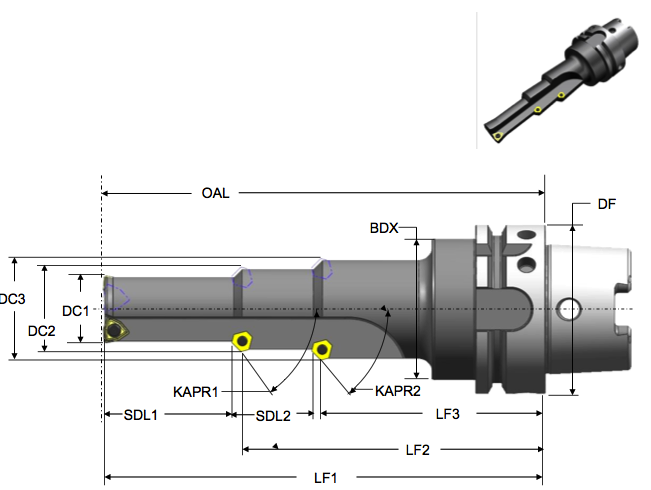
\includegraphics[width=0.6\textwidth]{figures/a1-cutting-tool-measurement-diagram-3.png}
  \caption{Cutting Tool Measurement Diagram 1
  \\ (Cutting Tool, Cutting Item, and Assembly Item – ISO 13399)}
  \label{fig:a1-cutting-tool-measurement-diagram-3}
\end{figure}
\FloatBarrier

\begin{figure}[ht]
  \centering
  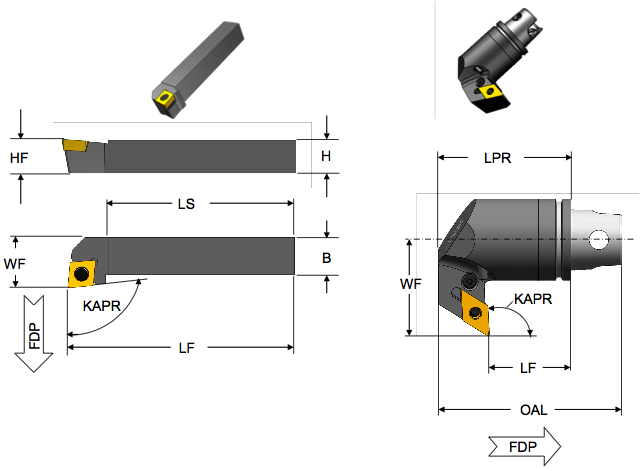
\includegraphics[width=0.6\textwidth]{figures/a2-cutting-tool-measurement-diagram-4.png}
  \caption{Cutting Tool Measurement Diagram 2
  \\  (Cutting Tool, Cutting Item, and Assembly Item – ISO 13399)}
  \label{fig:a2-cutting-tool-measurement-diagram-4}
\end{figure}
\FloatBarrier


\begin{figure}[ht]
  \centering
  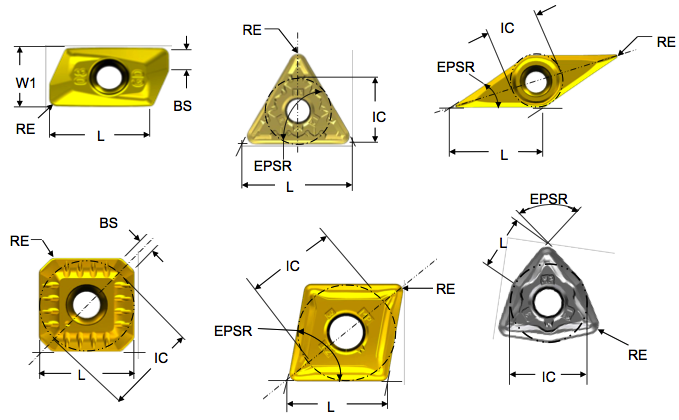
\includegraphics[width=0.6\textwidth]{figures/a3-cutting-item-measurement-diagram-3.png}
  \caption{Cutting Tool Measurement Diagram 3
  \\  (Cutting Item – ISO 13399)}
  \label{fig:a3-cutting-item-measurement-diagram-3}
\end{figure}
\FloatBarrier

\begin{figure}[ht]
  \centering
  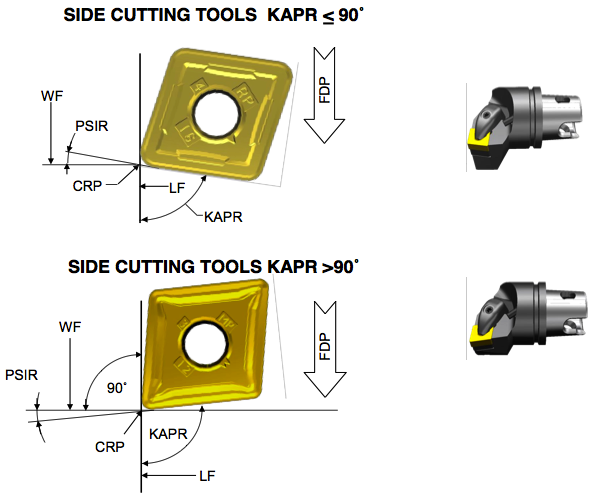
\includegraphics[width=0.6\textwidth]{figures/a4-cutting-item-measurement-diagram-4.png}
  \caption{Cutting Tool Measurement Diagram 4
  \\  (Cutting Item – ISO 13399)}
  \label{fig:a4-cutting-item-measurement-diagram-4}
\end{figure}
\FloatBarrier

\begin{figure}[ht]
  \centering
  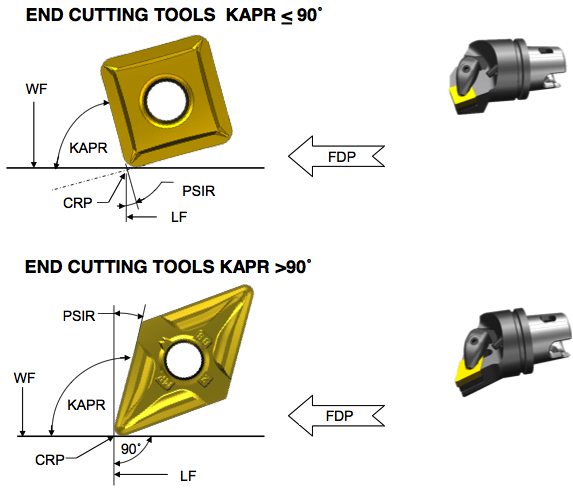
\includegraphics[width=0.6\textwidth]{figures/a5-cutting-item-measurement-diagram-5.png}
  \caption{Cutting Tool Measurement Diagram 5
  \\  (Cutting Item – ISO 13399)}
  \label{fig:a5-cutting-item-measurement-diagram-5}
\end{figure}
\FloatBarrier

\begin{figure}[ht]
  \centering
  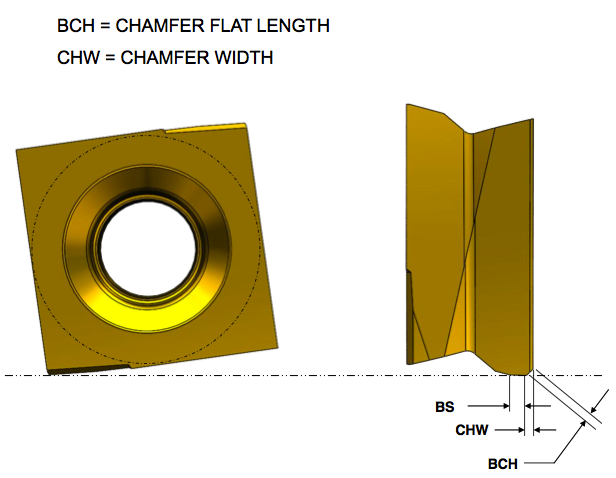
\includegraphics[width=0.6\textwidth]{figures/a6-cutting-item-measurement-diagram-6.png}
  \caption{Cutting Tool Measurement Diagram 6
  \\  (Cutting Item – ISO 13399)}
  \label{fig:a6-cutting-item-measurement-diagram-6}
\end{figure}
\FloatBarrier

\pagebreak

\subsection{Cutting Tool Example}

\subsubsection{Shell Mill}

\begin{figure}[ht]
  \centering
  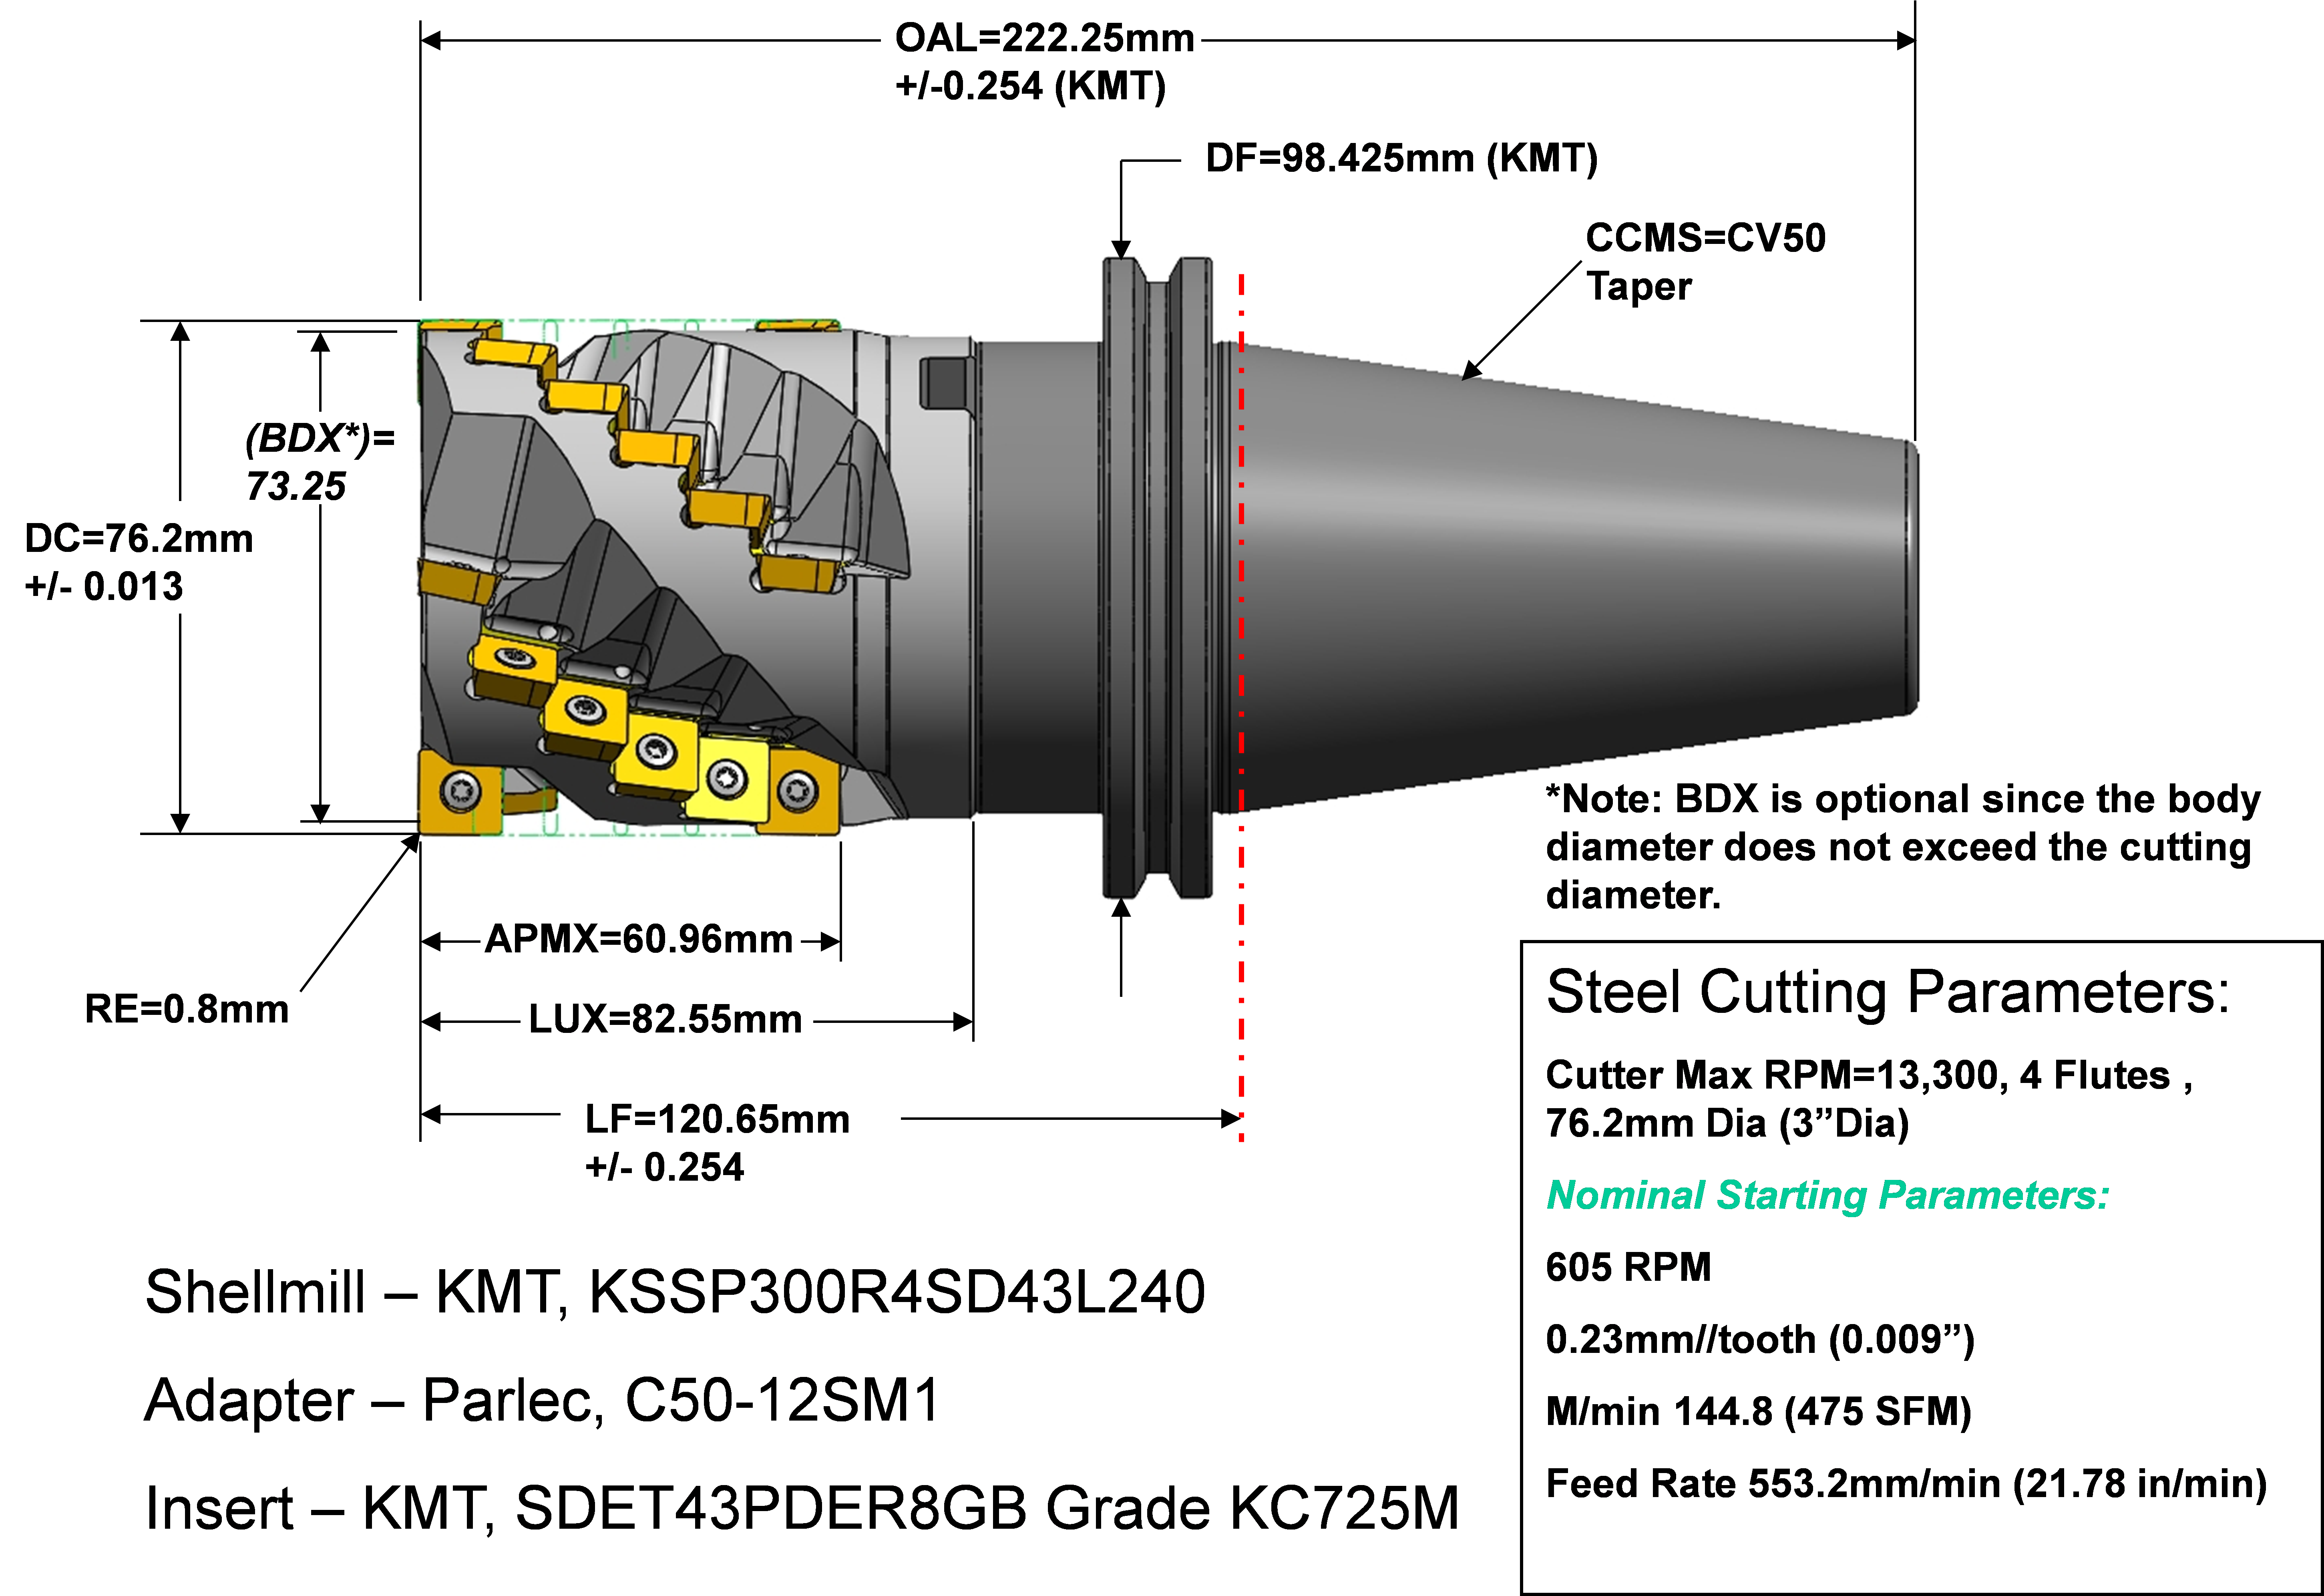
\includegraphics[width=0.6\textwidth]{figures/a7-shell-mill-side-view.png}
  \caption{Shell Mill Side View}
  \label{fig:a7-shell-mill-side-view}
\end{figure}
\FloatBarrier

\begin{figure}[ht]
  \centering
  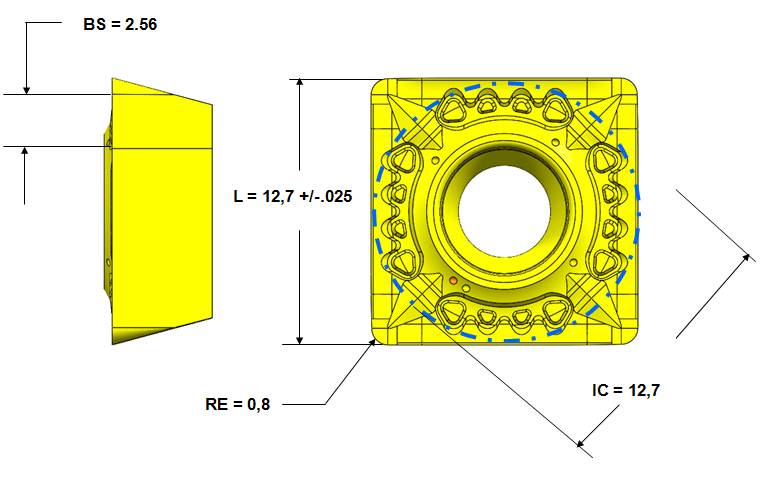
\includegraphics[width=0.6\textwidth]{figures/a8-indexable-insert-measurements.png}
  \caption{Indexable Insert Measurements}
  \label{fig:a8-indexable-insert-measurements}
\end{figure}
\FloatBarrier

\begin{lstlisting}[firstnumber=1,escapechar=|,% 
caption={Example for Indexable Insert Measurements}, label={lst:indexable-insert-measurements}]
<?xml version="1.0" encoding="UTF-8"?>
<MTConnectAssets 
xmlns:m="urn:mtconnect.org:MTConnectAssets:1.2" 
xmlns="urn:mtconnect.org:MTConnectAssets:1.2" 
xmlns:xsi="http://www.w3.org/2001/XMLSchema-instance" 
xsi:schemaLocation="urn:mtconnect.org:MTConnectAssets:1.2
http://mtconnect.org/schemas/MTConnectAssets\_1.2.xsd">
  <Header creationTime="2011-05-11T13:55:22" 
  assetBufferSize="1024" sender="localhost"
  assetCount="2" version="1.2" instanceId="1234"/>
  <Assets>
  <CuttingTool serialNumber="1" toolId="KSSP300R4SD43L240" 
  timestamp="2011-05-11T13:55:22" assetId="KSSP300R4SD43L240.1" 
  manufacturers="KMT,Parlec">
    <CuttingToolLifeCycle>
    <CutterStatus><Status>NEW</Status></CutterStatus>
    <ProcessSpindleSpeed maximum="13300" 
    nominal="605">10000</ProcessSpindleSpeed>
    <ProcessFeedRate
    nominal="9.22">9.22</ProcessSpindleSpeed>
    <ConnectionCodeMachineSide>CV50
    </ConnectionCodeMachineSide>
    <Measurements>
      <BodyDiameterMax code="BDX">73.25
      </BodyDiameterMax>
      <OverallToolLength nominal="222.25" 
        minimum="221.996" maximum="222.504" 
        code="OAL">222.25</OverallToolLength>
      <UsableLengthMax code="LUX" nominal="82.55">82.55
      </UsableLengthMax>
      <CuttingDiameterMax code="DC" nominal="76.2" 
        maximum="76.213" minimum="76.187">76.2
      </CuttingDiameterMax>
      <BodyLengthMax code="LF" nominal="120.65" 
        maximum="120.904" minimum="120.404">120.65
      </BodyLengthMax>
      <DepthOfCutMax code="APMX" 
      nominal="60.96">60.95</DepthOfCutMax>
      <FlangeDiameterMax code="DF" 
        nominal="98.425">98.425</FlangeDiameterMax>
    </Measurements>
    <CuttingItems count="24">
      <CuttingItem indices="1-24" itemId="SDET43PDER8GB" 
        manufacturers="KMT" grade="KC725M">
        <Measurements>
          <CuttingEdgeLength code="L" nominal="12.7" 
            minimum="12.675" maximum="12.725">12.7
          </CuttingEdgeLength>
        <WiperEdgeLength code="BS" nominal=
          "2.56">2.56</WiperEdgeLength>
        <IncribedCircleDiameter code="IC"
          nominal="12.7">12.7
        </IncribedCircleDiameter>
        <CornerRadius code="RE" nominal="0.8">
          0.8</CornerRadius>
      </Measurements>
      </CuttingItem>
    </CuttingItems>
    </CuttingToolLifeCycle>
    </CuttingTool>
  </Assets>
</MTConnectAssets>
\end{lstlisting}

\pagebreak

\subsubsection{Step Drill}

\begin{figure}[ht]
  \centering
  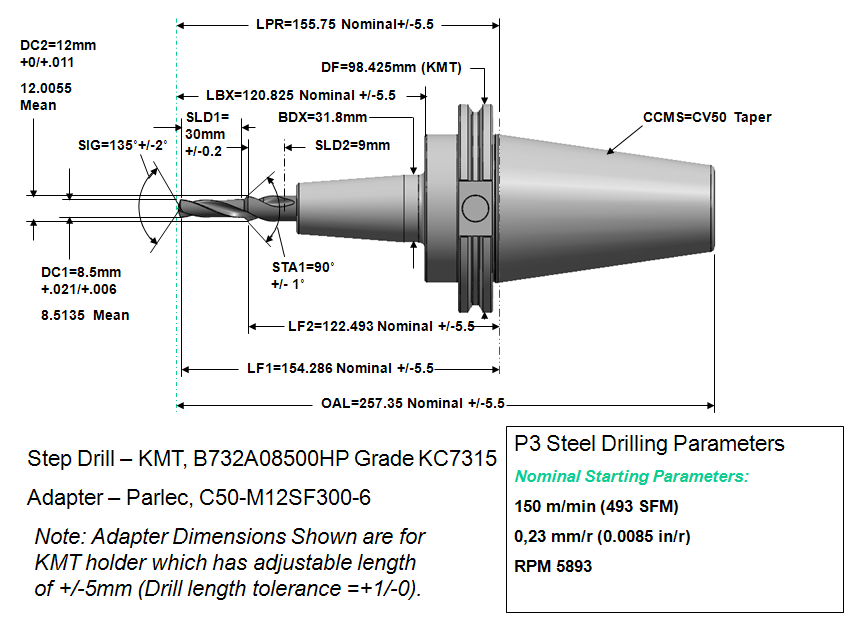
\includegraphics[width=0.6\textwidth]{figures/a9-step-drill-side-view.png}
  \caption{Step Mill Side View}
  \label{fig:a9-step-drill-side-view}
\end{figure}
\FloatBarrier

\begin{lstlisting}[firstnumber=1,escapechar=|,% 
caption={Example for Step Mill Side View}, label={lst:step-drill-side-view}]
<?xml version="1.0" encoding="UTF-8"?>
<MTConnectAssets xmlns:m="urn:mtconnect.org:MTConnectAssets:1.2" 
xmlns="urn:mtconnect.org:MTConnectAssets:1.2" 
xmlns:xsi="http://www.w3.org/2001/XMLSchema-instance" 
xsi:schemaLocation="urn:mtconnect.org:MTConnectAssets:1.2 
http://mtconnect.org/schemas/MTConnectAssets\_1.2.xsd">
  <Header creationTime="2011-05-
  11T13:55:22" assetBufferSize="1024" 
  sender="localhost" assetCount="2" version="1.2" instanceId="1234"/>
  <Assets>
    <CuttingTool serialNumber="1 " toolId="B732A08500HP" 
    timestamp="2011-05-11T13:55:22" assetId="B732A08500HP " 
    manufacturers="KMT,Parlec">
      <Description>
        Step Drill - KMT, B732A08500HP Grade KC7315
        Adapter - Parlec, C50-M12SF300-6
      </Description>
      <CuttingToolLifeCycle>
        <CutterStatus><Status>NEW</Status></CutterStatus>
        <ProcessSpindleSpeed nominal="5893">5893</ProcessSpindleSpeed>
        <ProcessFeedRate nominal="2.5">2.5</ProcessFeedRate>
        <ConnectionCodeMachineSide>CV50 Taper</ConnectionCodeMachineSide>
        <Measurements>
          <BodyDiameterMax code="BDX">31.8</BodyDiameterMax>
          <BodyLengthMax code="LBX" nominal="120.825" maximum="126.325" 
          minimum="115.325">120.825</BodyLengthMax>
          <ProtrudingLength code="LPR" nominal="155.75" maximum="161.25" 
          minimum="150.26">155.75</ProtrudingLength>
          <FlangeDiameterMax code="DF" 
          nominal="98.425">98.425</FlangeDiameterMax>
          <OverallToolLength nominal="257.35" minimum="251.85" 
          maximum="262.85" code="OAL">257.35</OverallToolLength>
        </Measurements>
        <CuttingItems count="2">
          <CuttingItem indices="1" manufacturers="KMT" grade="KC7315">>
            <Measurements>
              <CuttingDiameter code="DC1" nominal="8.5" maximum="8.521" 
              minimum="8.506">8.5135</CuttingDiameter>
              <StepIncludedAngle code="STA1" nominal="90" maximum="91" 
              minimum="89">90</StepIncludedAngle>
              <FunctionalLength code="LF1" nominal="154.286" 
              minimum="148.786" 
              maximum="159.786">154.286</FunctionalLength>
              <StepDiameterLength code="SDL1" 
              nominal="9">9</StepDiameterLength>
              <PointAngle code="SIG" nominal="135" minimum="133" 
              maximum="137">135</PointAngle>
            </Measurements>
          </CuttingItem>
          <CuttingItem indices="2" manufacturers="KMT" grade="KC7315">>
            <Measurements>
              <CuttingDiameter code="DC2" nominal="12" maximum="12.011" 
              minimum="12">12</CuttingDiameter>
              <FunctionalLength code="LF2" nominal="122.493" 
              maximum="127.993" 
              minimum="116.993">122.493</FunctionalLength>
              <StepDiameterLength code="SDL2" 
              nominal="9">9</StepDiameterLength>
            </Measurements>
          </CuttingItem>
        </CuttingItems>
      </CuttingToolLifeCycle>
    </CuttingTool>
  </Assets>
</MTConnectAssets>
\end{lstlisting}

\pagebreak

\subsubsection{Shell Mill with Individual Loci}

\begin{figure}[ht]
  \centering
  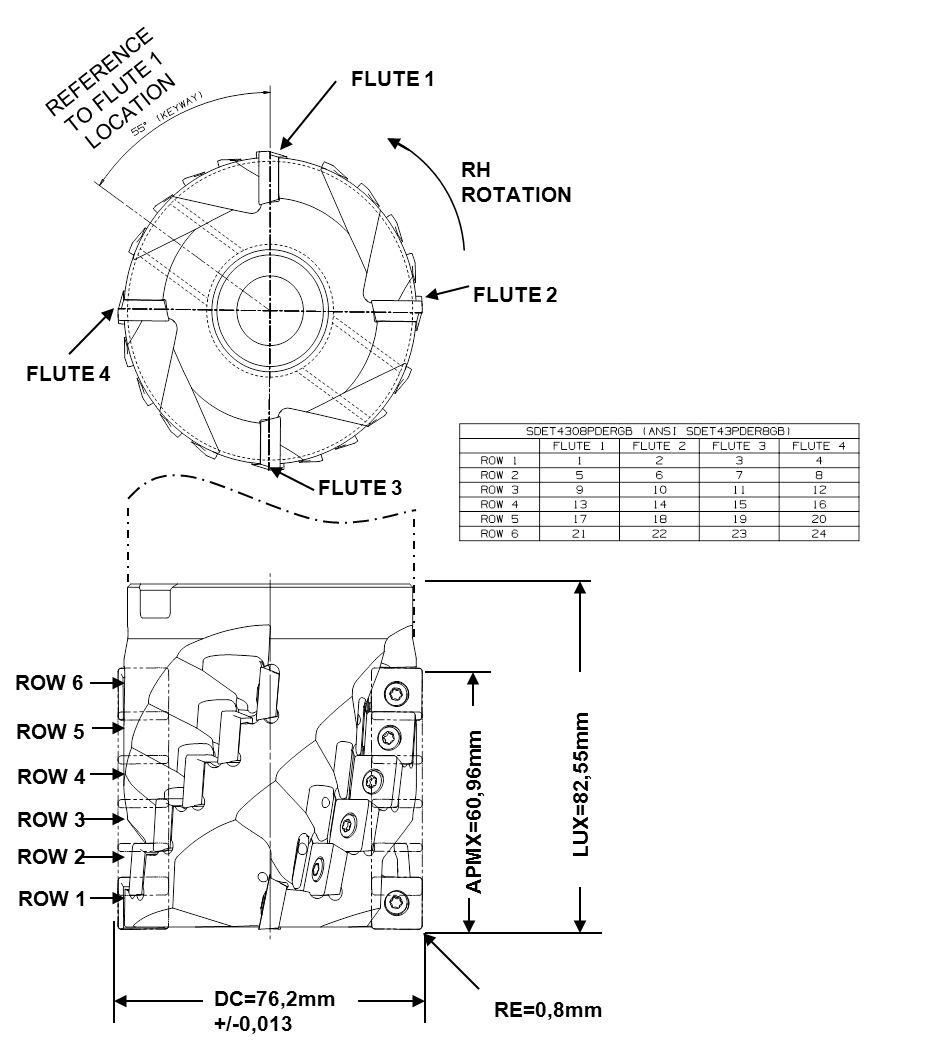
\includegraphics[width=0.6\textwidth]{figures/a10-shell-mill-with-explicate-loci.png}
  \caption{Shell Mill with Explicate Loci}
  \label{fig:a10-shell-mill-with-explicate-loci}
\end{figure}
\FloatBarrier

\begin{lstlisting}[firstnumber=1,escapechar=|,% 
caption={Example for Shell Mill with Explicate Loci}, label={lst:shell-mill-with-explicate-loci}]
<?xml version="1.0" encoding="UTF-8"?>
<MTConnectAssets xmlns:m="urn:mtconnect.org:MTConnectAssets:1.2" 
xmlns="urn:mtconnect.org:MTConnectAssets:1.2" 
xmlns:xsi="http://www.w3.org/2001/XMLSchema-instance" 
xsi:schemaLocation="urn:mtconnect.org:MTConnectAssets:1.2 
http://mtconnect.org/schemas/MTConnectAssets\_1.2.xsd">
  <Header creationTime="2011-05-11T13:55:22" assetBufferSize="1024" 
  sender="localhost" assetCount="2" version="1.2" instanceId="1234"/>
  <Assets>
    <CuttingTool serialNumber="1" toolId="KSSP300R4SD43L240" 
    timestamp="2011-05-11T13:55:22" assetId="KSSP300R4SD43L240.1" 
    manufacturers="KMT,Parlec">
      <Description>Keyway: 55 degrees</Description>
      <CuttingToolLifeCycle>
        <CutterStatus><Status>NEW</Status></CutterStatus>
        <Measurements>
          <UsableLengthMax code="LUX" 
          nominal="82.55">82.55</UsableLengthMax>
          <CuttingDiameterMax code="DC" nominal="76.2" maximum="76.213" 
          minimum="76.187">76.2</CuttingDiameterMax>
          <DepthOfCutMax code="APMX" nominal="60.96">60.95</DepthOfCutMax>
        </Measurements>
        <CuttingItems count="24">
          <CuttingItem indices="1" itemId="SDET43PDER8GB" 
          manufacturers="KMT">
            <Locus>FLUTE: 1, ROW: 1</Locus>
            <Measurements>
             <DriveAngle code="DRVA" nominal="55">55</DriveAngle>
           </Measurements>
          </CuttingItem>
          <CuttingItem indices="2-24" itemId="SDET43PDER8GB" 
          manufacturers="KMT">
            <Locus>FLUTE: 2-4, ROW: 1; FLUTE: 1-4, ROW 2-6</Locus>
          </CuttingItem>
        </CuttingItems>
      </CuttingToolLifeCycle>
    </CuttingTool>
  </Assets>
</MTConnectAssets>
\end{lstlisting}

\pagebreak

\subsubsection{Drill with Individual Loci}

\begin{figure}[ht]
  \centering
  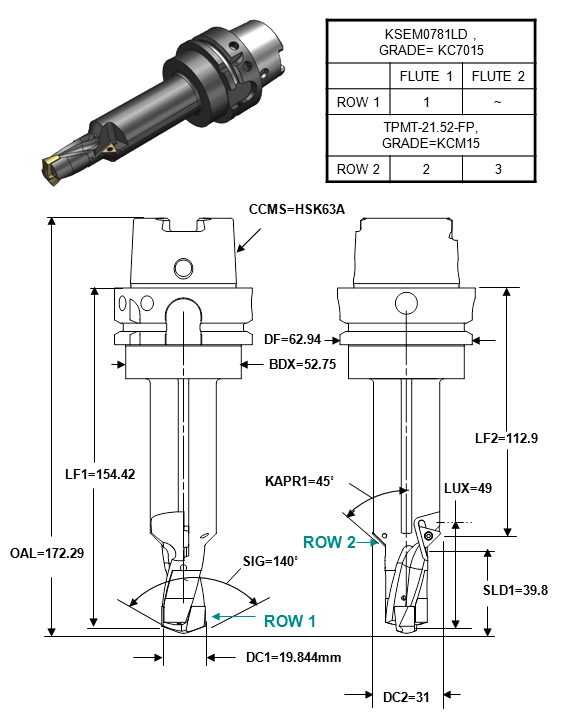
\includegraphics[width=0.6\textwidth]{figures/a11-step-drill-with-explicate-loci.png}
  \caption{Step Drill with Explicate Loci}
  \label{fig:a11-step-drill-with-explicate-loci}
\end{figure}
\FloatBarrier

\begin{lstlisting}[firstnumber=1,escapechar=|,% 
caption={Example for Step Drill with Explicate Loci}, label={lst:step-drill-with-explicate-loci}]
<?xml version="1.0" encoding="UTF-8"?>
<MTConnectAssets xmlns:m="urn:mtconnect.org:MTConnectAssets:1.2" 
xmlns="urn:mtconnect.org:MTConnectAssets:1.2" 
xmlns:xsi="http://www.w3.org/2001/XMLSchema-instance" 
xsi:schemaLocation="urn:mtconnect.org:MTConnectAssets:1.2 
http://mtconnect.org/schemas/MTConnectAssets\_1.2.xsd">
  <Header creationTime="2011-05-11T13:55:22" assetBufferSize="1024" 
  sender="localhost" assetCount="2" version="1.2" instanceId="1234"/>
  <Assets>
    <CuttingTool serialNumber="1" toolId="KSEM0781LD" 
    timestamp="2011-05-11T13:55:22" assetId="KSEM0781LD.1" manufacturers="KMT">
      <CuttingToolLifeCycle>
        <CutterStatus><Status>NEW</Status></CutterStatus>
        <ConnectionCodeMachineSide>HSK63A</ConnectionCodeMachineSide>
        <Measurements>
          <BodyDiameterMax code="BDX">52.75</BodyDiameterMax>
          <OverallToolLength nominal="172.29" 
          code="OAL">172.29</OverallToolLength>
          <UsableLengthMax code="LUX" nominal="49">49</UsableLengthMax>
          <FlangeDiameterMax code="DF" 
          nominal="62.94">62.94</FlangeDiameterMax>
        </Measurements>
        <CuttingItems count="3">
          <CuttingItem indices="1" itemId="KSEM0781LD" manufacturers="KMT" 
          grade="KC7015">
            <Locus>FLUTE: 1, ROW: 1</Locus>
            <Measurements>
         <FunctionalLength code="LF1" nominal="154.42">154.42</FunctionalLength>
         <CuttingDiameter code="DC1" nominal="19.844">19.844</CuttingDiameter>
         <PointAngle code="SIG" nominal="140">140</PointAngle>
         <ToolCuttingEdgeAngle code="KAPR1" nominal="45">45</ToolCuttingEdgeAngle>
         <StepDiameterLength code="SLD1" nominal="39.8">39.8</StepDiameterLength>
            </Measurements>
          </CuttingItem>
          <CuttingItem indices="2-3" itemId="TPMT-21.52-FP" 
          manufacturers="KMT" grade="KCM15">
            <Locus>FLUTE: 1-2, ROW: 2</Locus>
            <Measurements>
         <FunctionalLength code="LF2" nominal="112.9">119.2</FunctionalLength>
         <CuttingDiameter code="DC2" nominal="31">31</CuttingDiameter>
            </Measurements>
          </CuttingItem>
        </CuttingItems>
      </CuttingToolLifeCycle>
    </CuttingTool>
  </Assets>
</MTConnectAssets>
\end{lstlisting}

\pagebreak

\subsubsection{Shell Mill with Different Inserts on First Row}

\begin{figure}[ht]
  \centering
  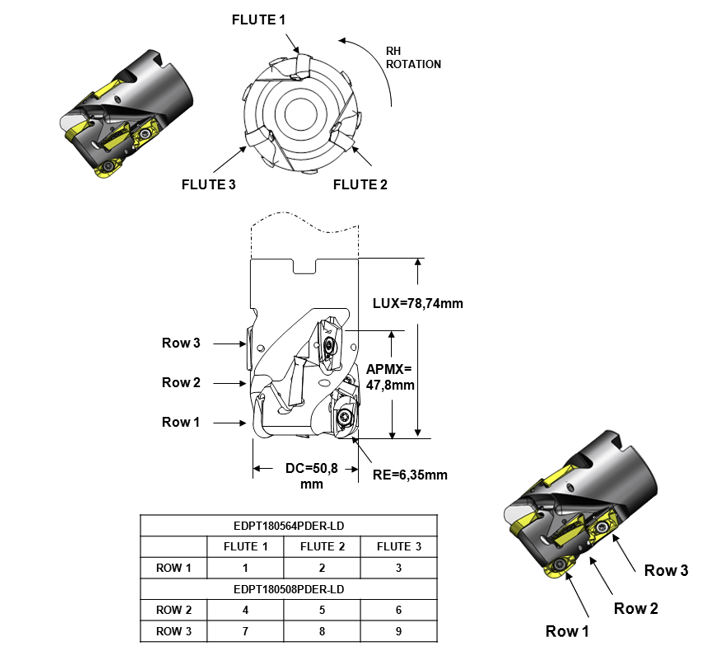
\includegraphics[width=0.6\textwidth]{figures/a12-shell-mill-with-different-inserts-on-first-row.png}
  \caption{Shell Mill with Different Inserts on First Row}
  \label{fig:a12-shell-mill-with-different-inserts-on-first-row.png}
\end{figure}
\FloatBarrier

\begin{lstlisting}[firstnumber=1,escapechar=|,% 
caption={Example for Shell Mill with Different Inserts on First Row}, label={lst:shell-mill-with-different-inserts-on-first-row}]
<?xml version="1.0" encoding="UTF-8"?>
<MTConnectAssets xmlns:m="urn:mtconnect.org:MTConnectAssets:1.2" 
xmlns="urn:mtconnect.org:MTConnectAssets:1.2" 
xmlns:xsi="http://www.w3.org/2001/XMLSchema-instance" 
xsi:schemaLocation="urn:mtconnect.org:MTConnectAssets:1.2 
http://mtconnect.org/schemas/MTConnectAssets\_1.2.xsd">
  <Header creationTime="2011-05-11T13:55:22" assetBufferSize="1024" 
  sender="localhost" assetCount="2" version="1.2" instanceId="1234"/>
  <Assets>
    <CuttingTool serialNumber="1" toolId="XXX" timestamp="2011-05-11T13:55:22" 
    assetId="XXX.1" manufacturers="KMT">
      <CuttingToolLifeCycle>
        <CutterStatus><Status>NEW</Status></CutterStatus>
        <Measurements>
          <DepthOfCutMax code="APMX" nominal="47.8">47.8</DepthOfCutMax>
          <CuttingDiameterMax code="DC" 
          nominal="50.8">50.8</CuttingDiameterMax>
          <UsableLengthMax code="LUX" 
          nominal="78.74">78.74</UsableLengthMax>
        </Measurements>
        <CuttingItems count="9">
          <CuttingItem indices="1-3" itemId="EDPT180564PDER-LD" 
          manufacturers="KMT">
            <Locus>FLUTE: 1-3, ROW: 1</Locus>
            <Measurements>
              <CornerRadius code="RE" nominal="6.25">6.35</CornerRadius>
            </Measurements>
          </CuttingItem>
          <CuttingItem indices="4-9" itemId="EDPT180508PDER-LD" 
          manufacturers="KMT">
            <Locus>FLANGE: 1-4, ROW: 2-3</Locus>
          </CuttingItem>
        </CuttingItems>
      </CuttingToolLifeCycle>
    </CuttingTool>
  </Assets>
</MTConnectAssets>
\end{lstlisting}